\documentclass[%
 reprint,
 superscriptaddress,
 amsmath,
 amssymb,
 prstab,
]{revtex4-1}

\usepackage{graphicx}% Include figure files
\usepackage{dcolumn}% Align table columns on decimal point
\usepackage{bm}% bold math
\maxdeadcycles=200

\begin{document}

\title{Design and Commissioning of the CTF3 Phase Feedforward System}

\author{J.~Roberts}
\email{Corresponding author Jack.Roberts@cern.ch}
\affiliation{John Adams Institute (JAI), University of Oxford, Denys Wilkinson 
Building, Keble Road, Oxford, OX1 3RH, United Kingdom}
\affiliation{The European Organization for Nuclear Research (CERN), Geneva 23, 
CH-1211, Switzerland}

\author{P.~Skowronski}
\affiliation{The European Organization for Nuclear Research (CERN), Geneva 23, 
	CH-1211, Switzerland}

\author{P.~Burrows}
\affiliation{John Adams Institute (JAI), University of Oxford, Denys Wilkinson 
Building, Keble Road, Oxford, OX1 3RH, United Kingdom}

\author{G.~Christian}
\affiliation{John Adams Institute (JAI), University of Oxford, Denys Wilkinson 
Building, Keble Road, Oxford, OX1 3RH, United Kingdom}

\author{R.~Corsini}
\affiliation{The European Organization for Nuclear Research (CERN), Geneva 23, 
CH-1211, Switzerland}

\author{A.~Ghigo}
\affiliation{Laboratori Nazionali di Frascati (LNFN), Via Enrico Fermi, 40, 
00044 
Frascati RM, Italy}

\author{F.~Marcellini}
\affiliation{Laboratori Nazionali di Frascati (LNFN), Via Enrico Fermi, 40, 
00044 
Frascati RM, Italy}

\author{C.~Perry}
\affiliation{John Adams Institute (JAI), University of Oxford, Denys Wilkinson 
Building, Keble Road, Oxford, OX1 3RH, United Kingdom}


\date{\today}

\begin{abstract}
Abstract
\end{abstract}

\maketitle

\section{\label{sec:intro}Introduction}

\begin{figure*}
	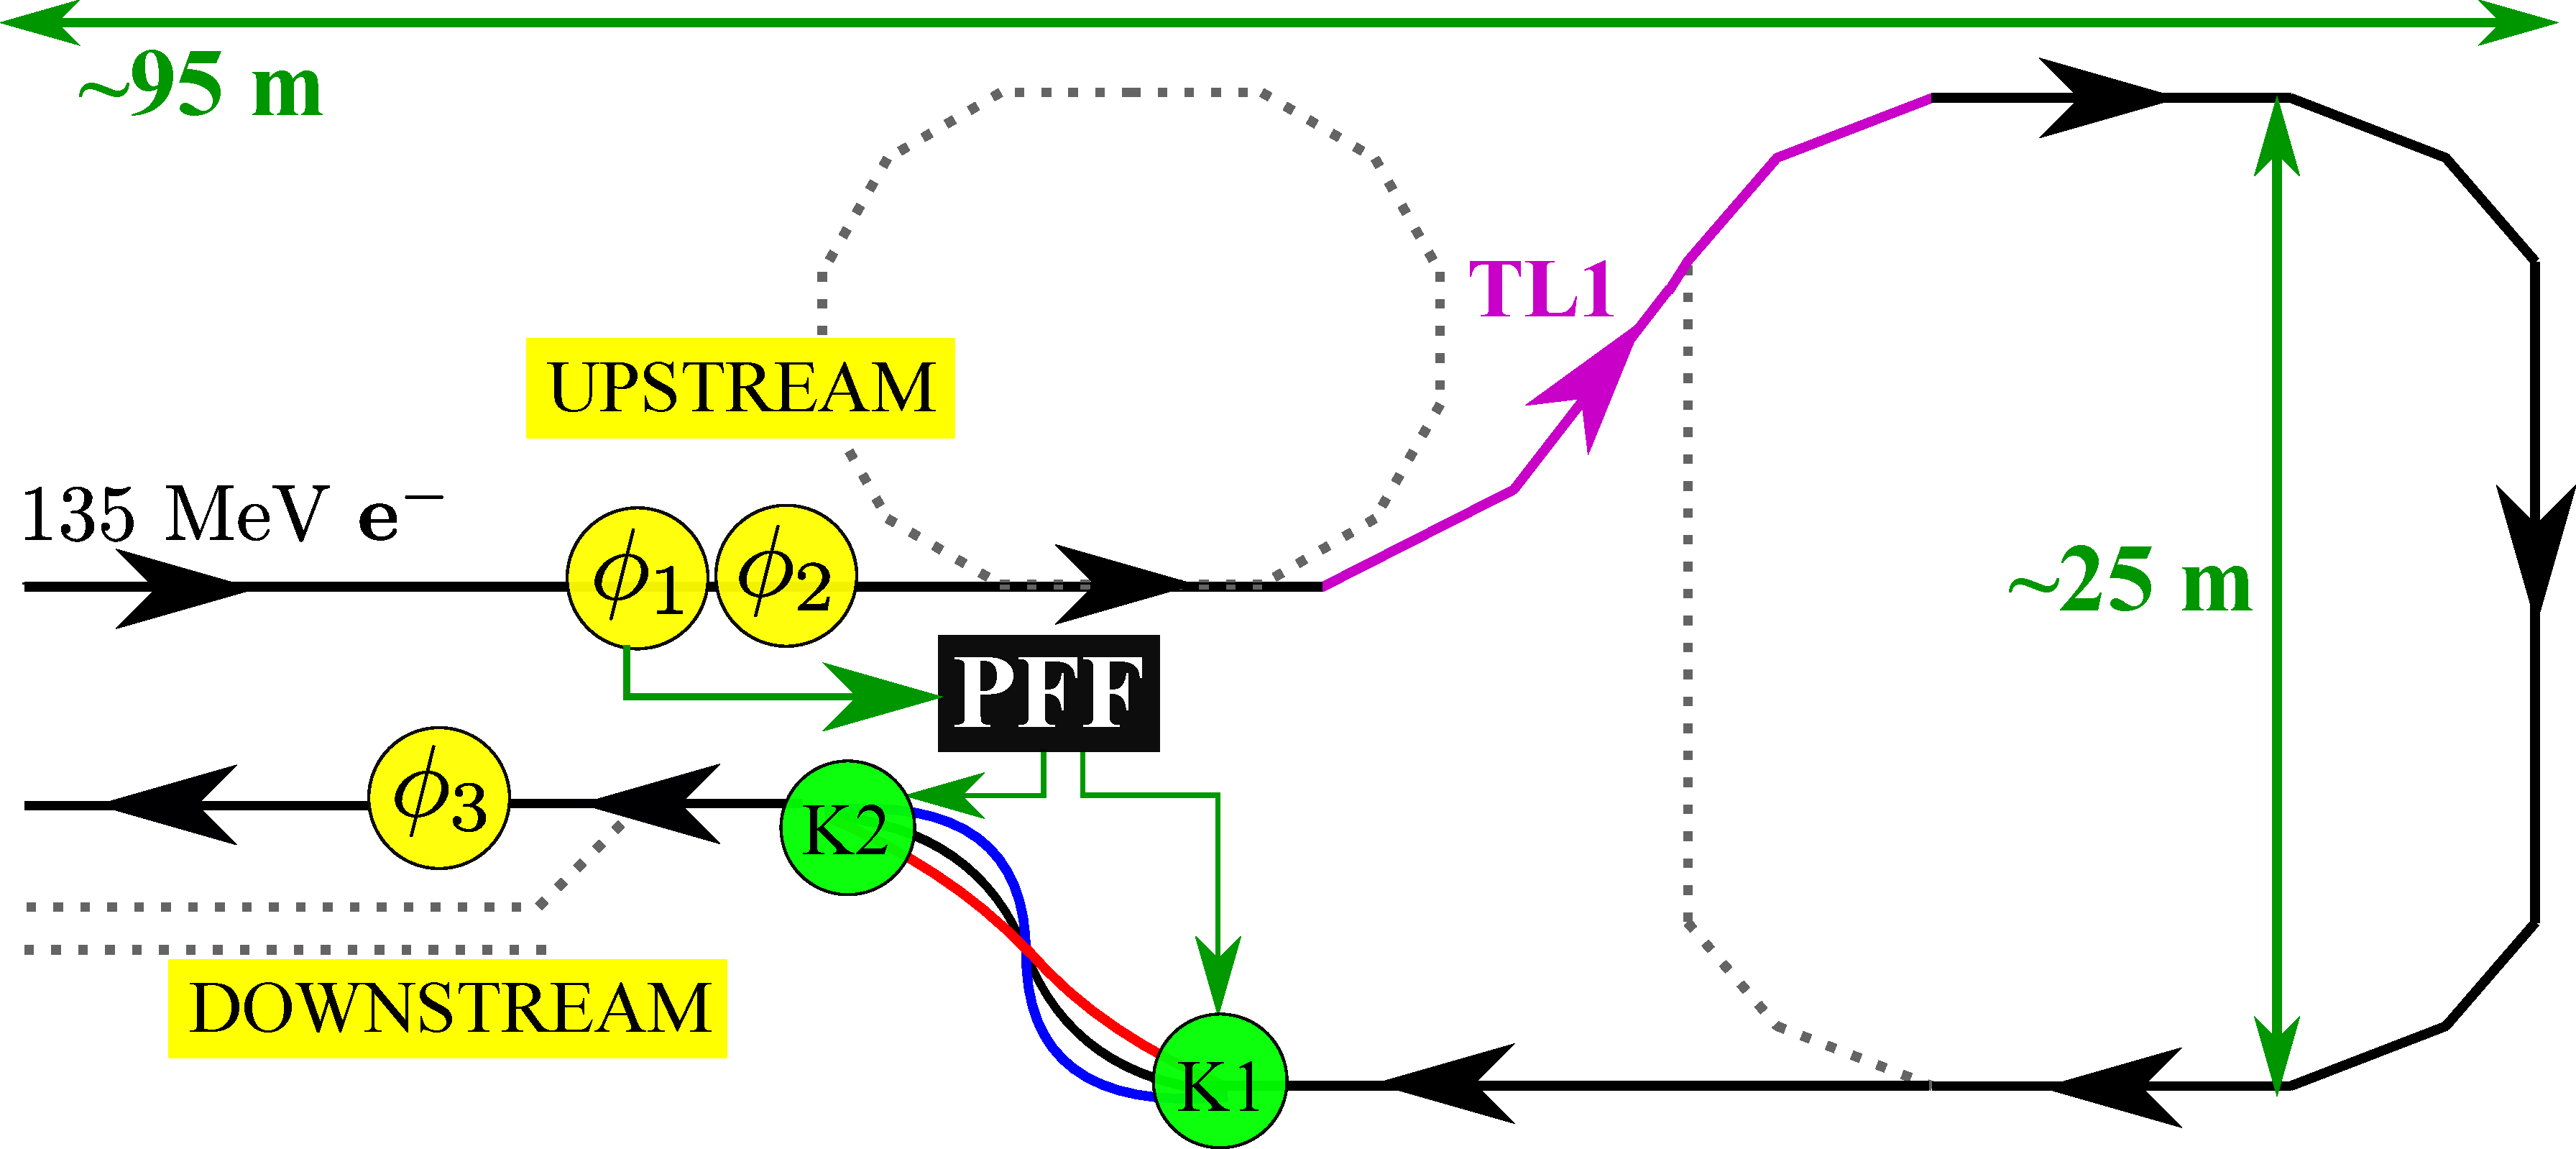
\includegraphics[width=\textwidth]{figs/intro/ctfpffLayout}% Here is 
	%how to 
	%import EPS art
	\caption{\label{f:pffLayout}Schematic of the PFF prototype at CTF3, 
	showing the phase monitors (\(\phi_1\) , 
	\(\phi_2\) and \(\phi_3\)) and kickers (K1 and K2). The black box “PFF” 
	represents the calculation and output of the correction, including the 
	phase monitor electronics, feedforward controller and kicker amplifiers.
	Dashed lines indicate beam lines that are not used during PFF operation. 
	Bunches arriving early at the upstream monitor (\(\phi_1\)) are directed 
	on to longer trajectories in the correction chicane (blue), and bunches 
	arriving late on to shorter trajectories (red).
		}
\end{figure*}

\section{\label{s:hw}Hardware}

\subsection{\label{ss:phMon}Phase Monitors}

\begin{figure}
	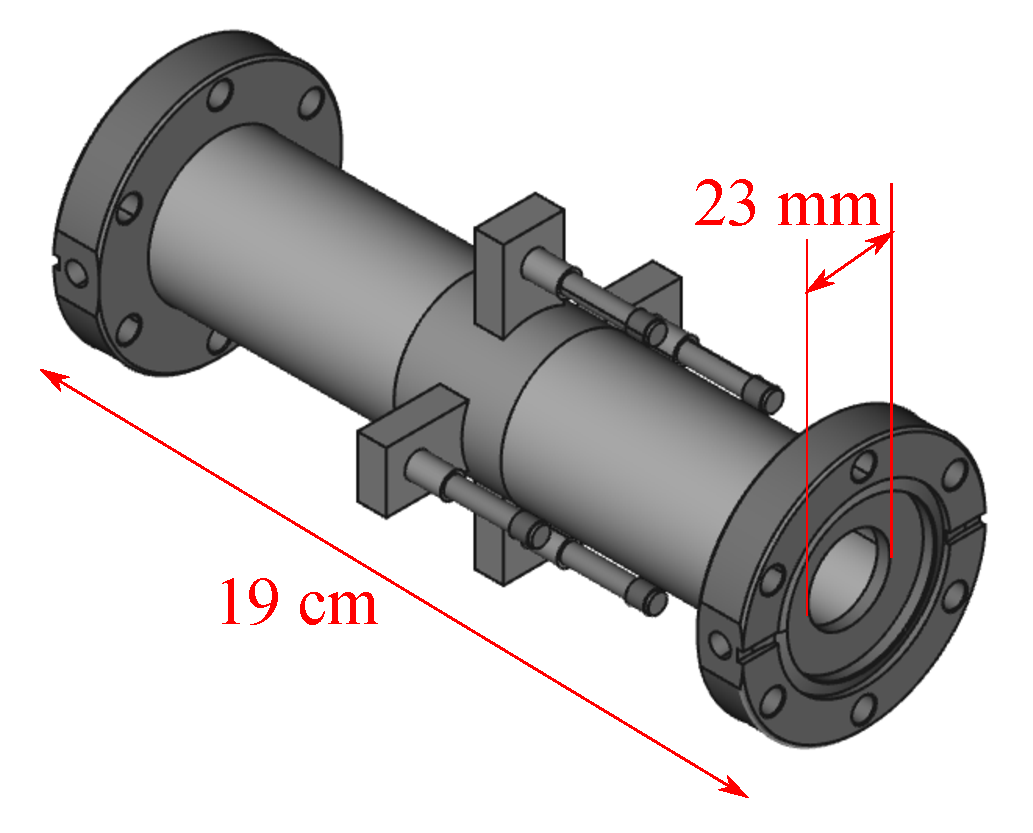
\includegraphics[width=\columnwidth]{figs/hw/phMonTechDraw}% Here is 
	%how to 
	%import EPS art
	\caption{\label{f:phMonTechDraw}
	}
\end{figure}

\begin{figure*}
	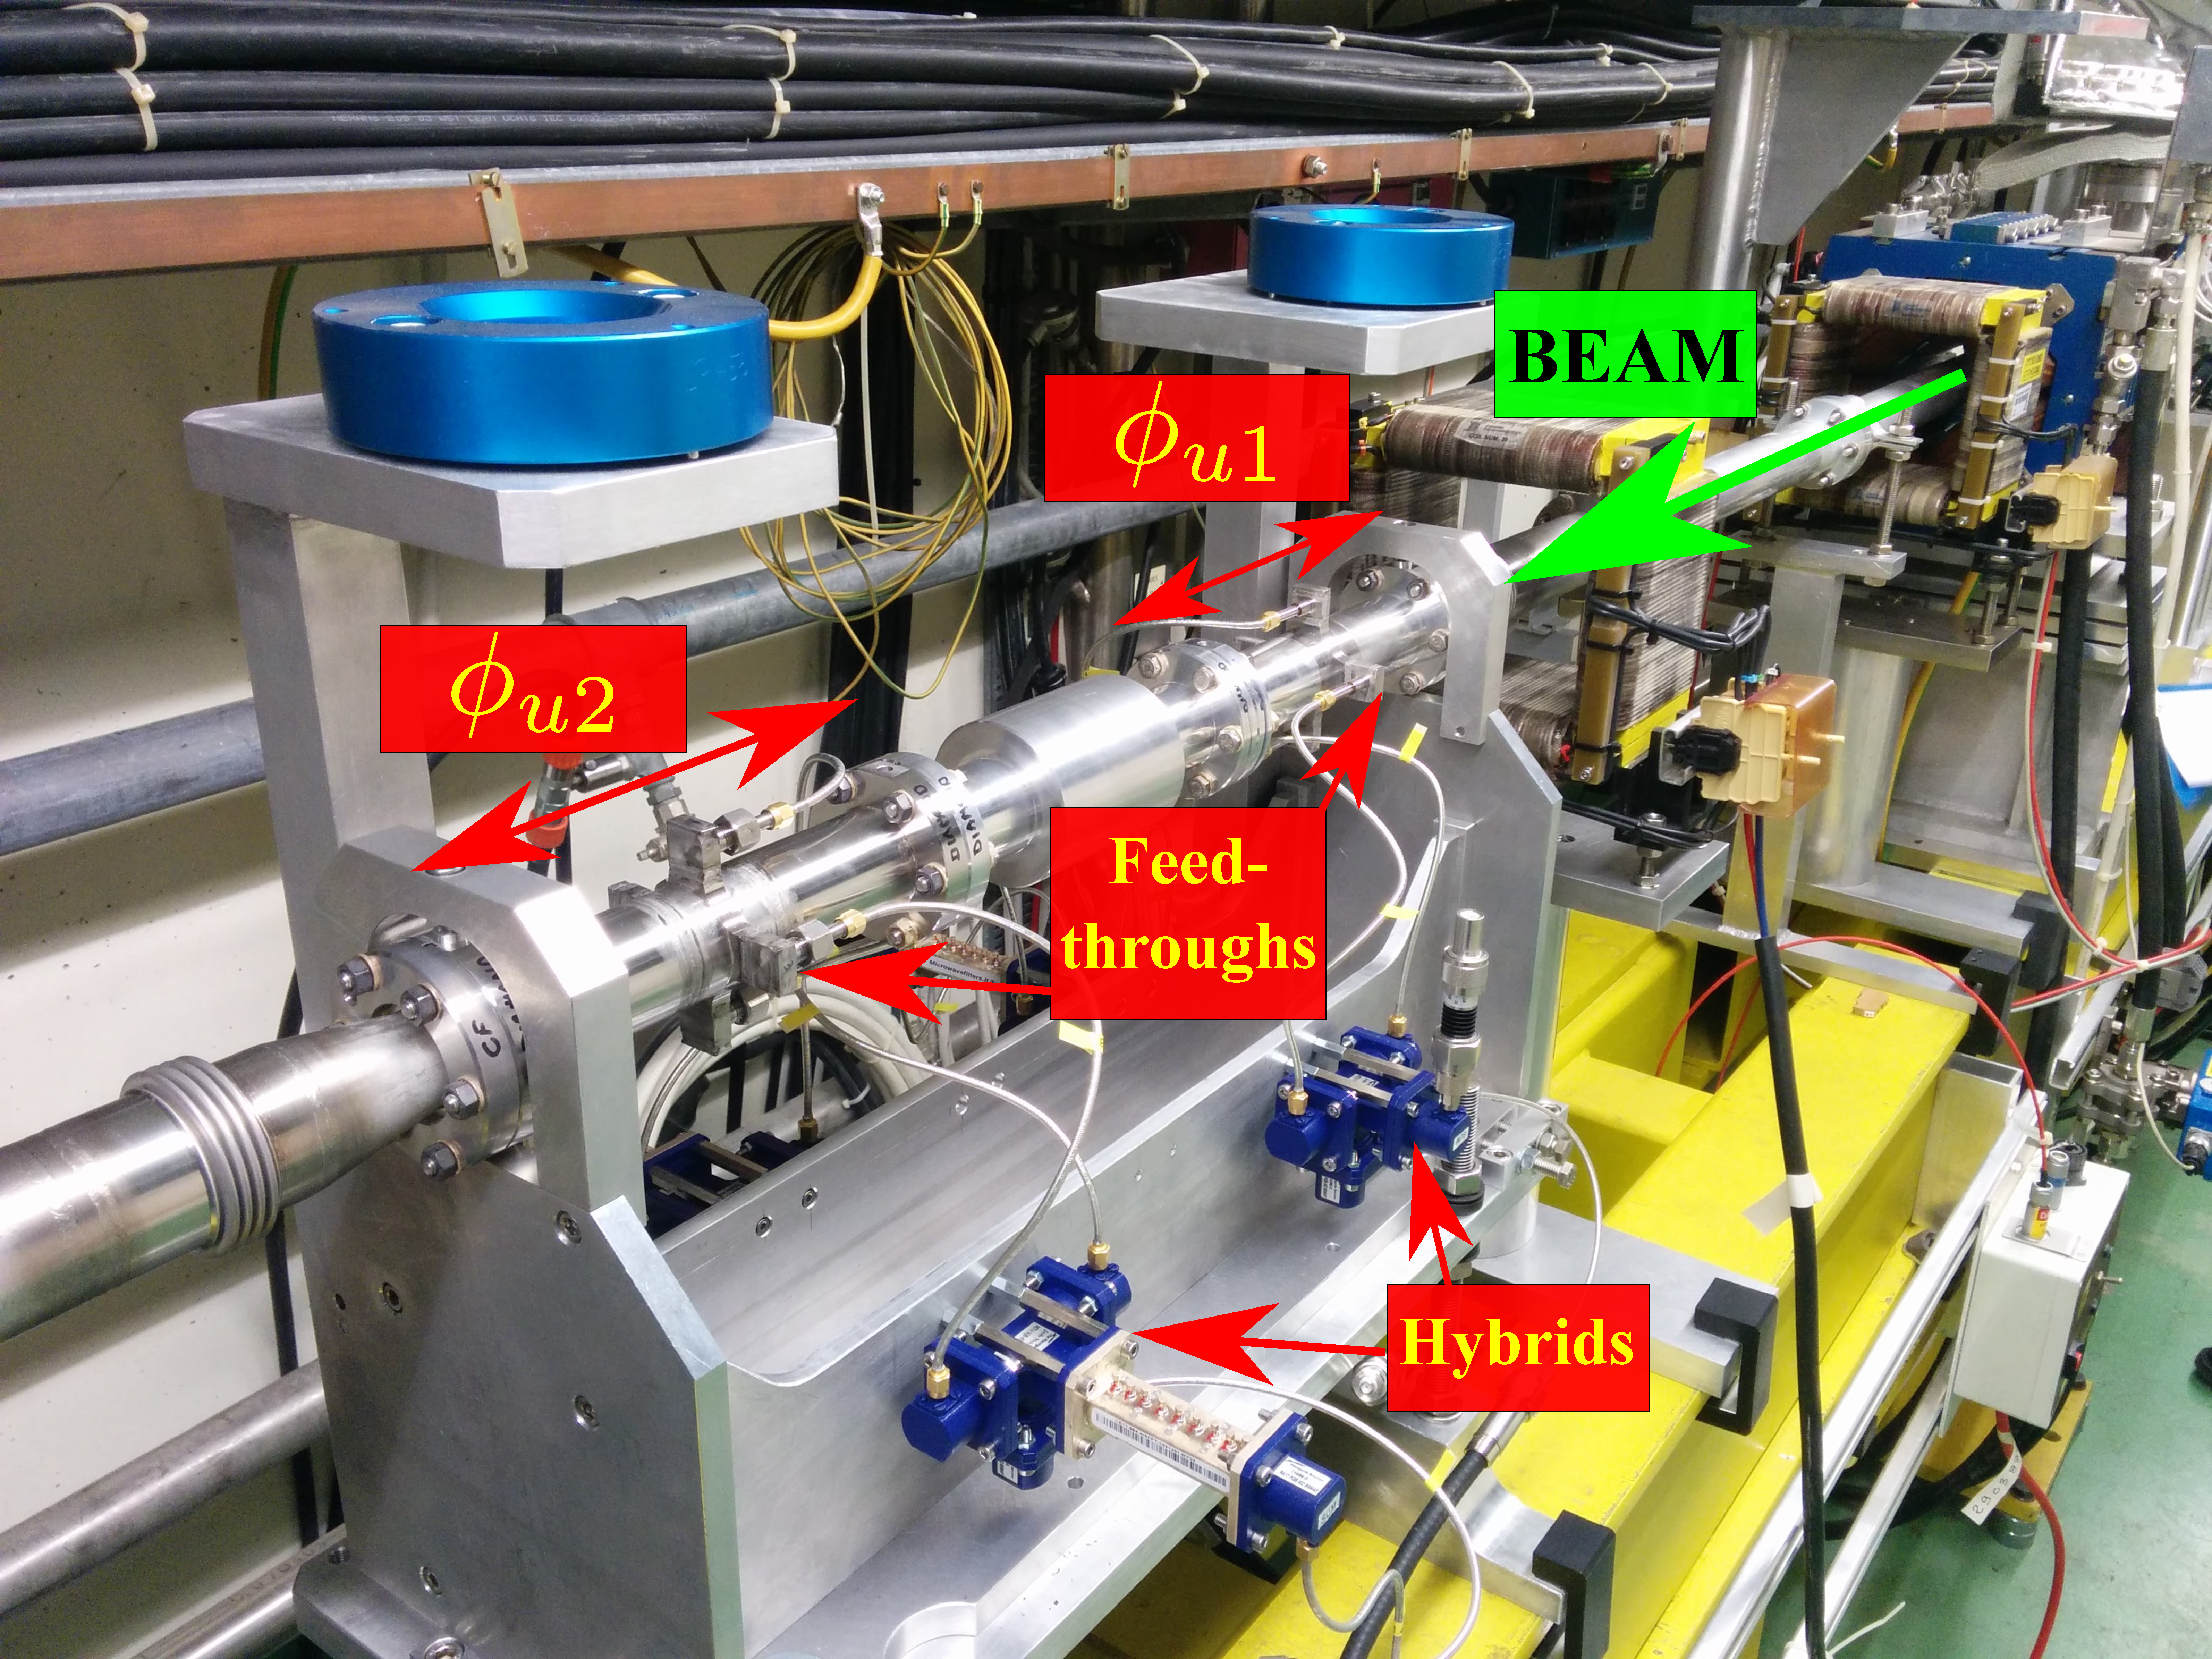
\includegraphics[width=\textwidth]{figs/hw/phMonCTPic}% Here is 
	%how to 
	%import EPS art
	\caption{\label{f:phMonCTPic}
	}
\end{figure*}

\begin{figure*}
	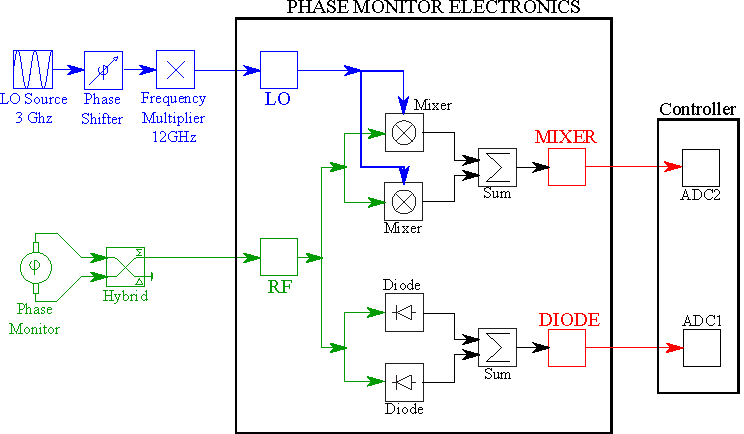
\includegraphics[width=\textwidth]{figs/hw/phMonDiagram}% Here is 
	%how to 
	%import EPS art
	\caption{\label{f:phMonDiagram}
	}
\end{figure*}

\begin{figure*}
	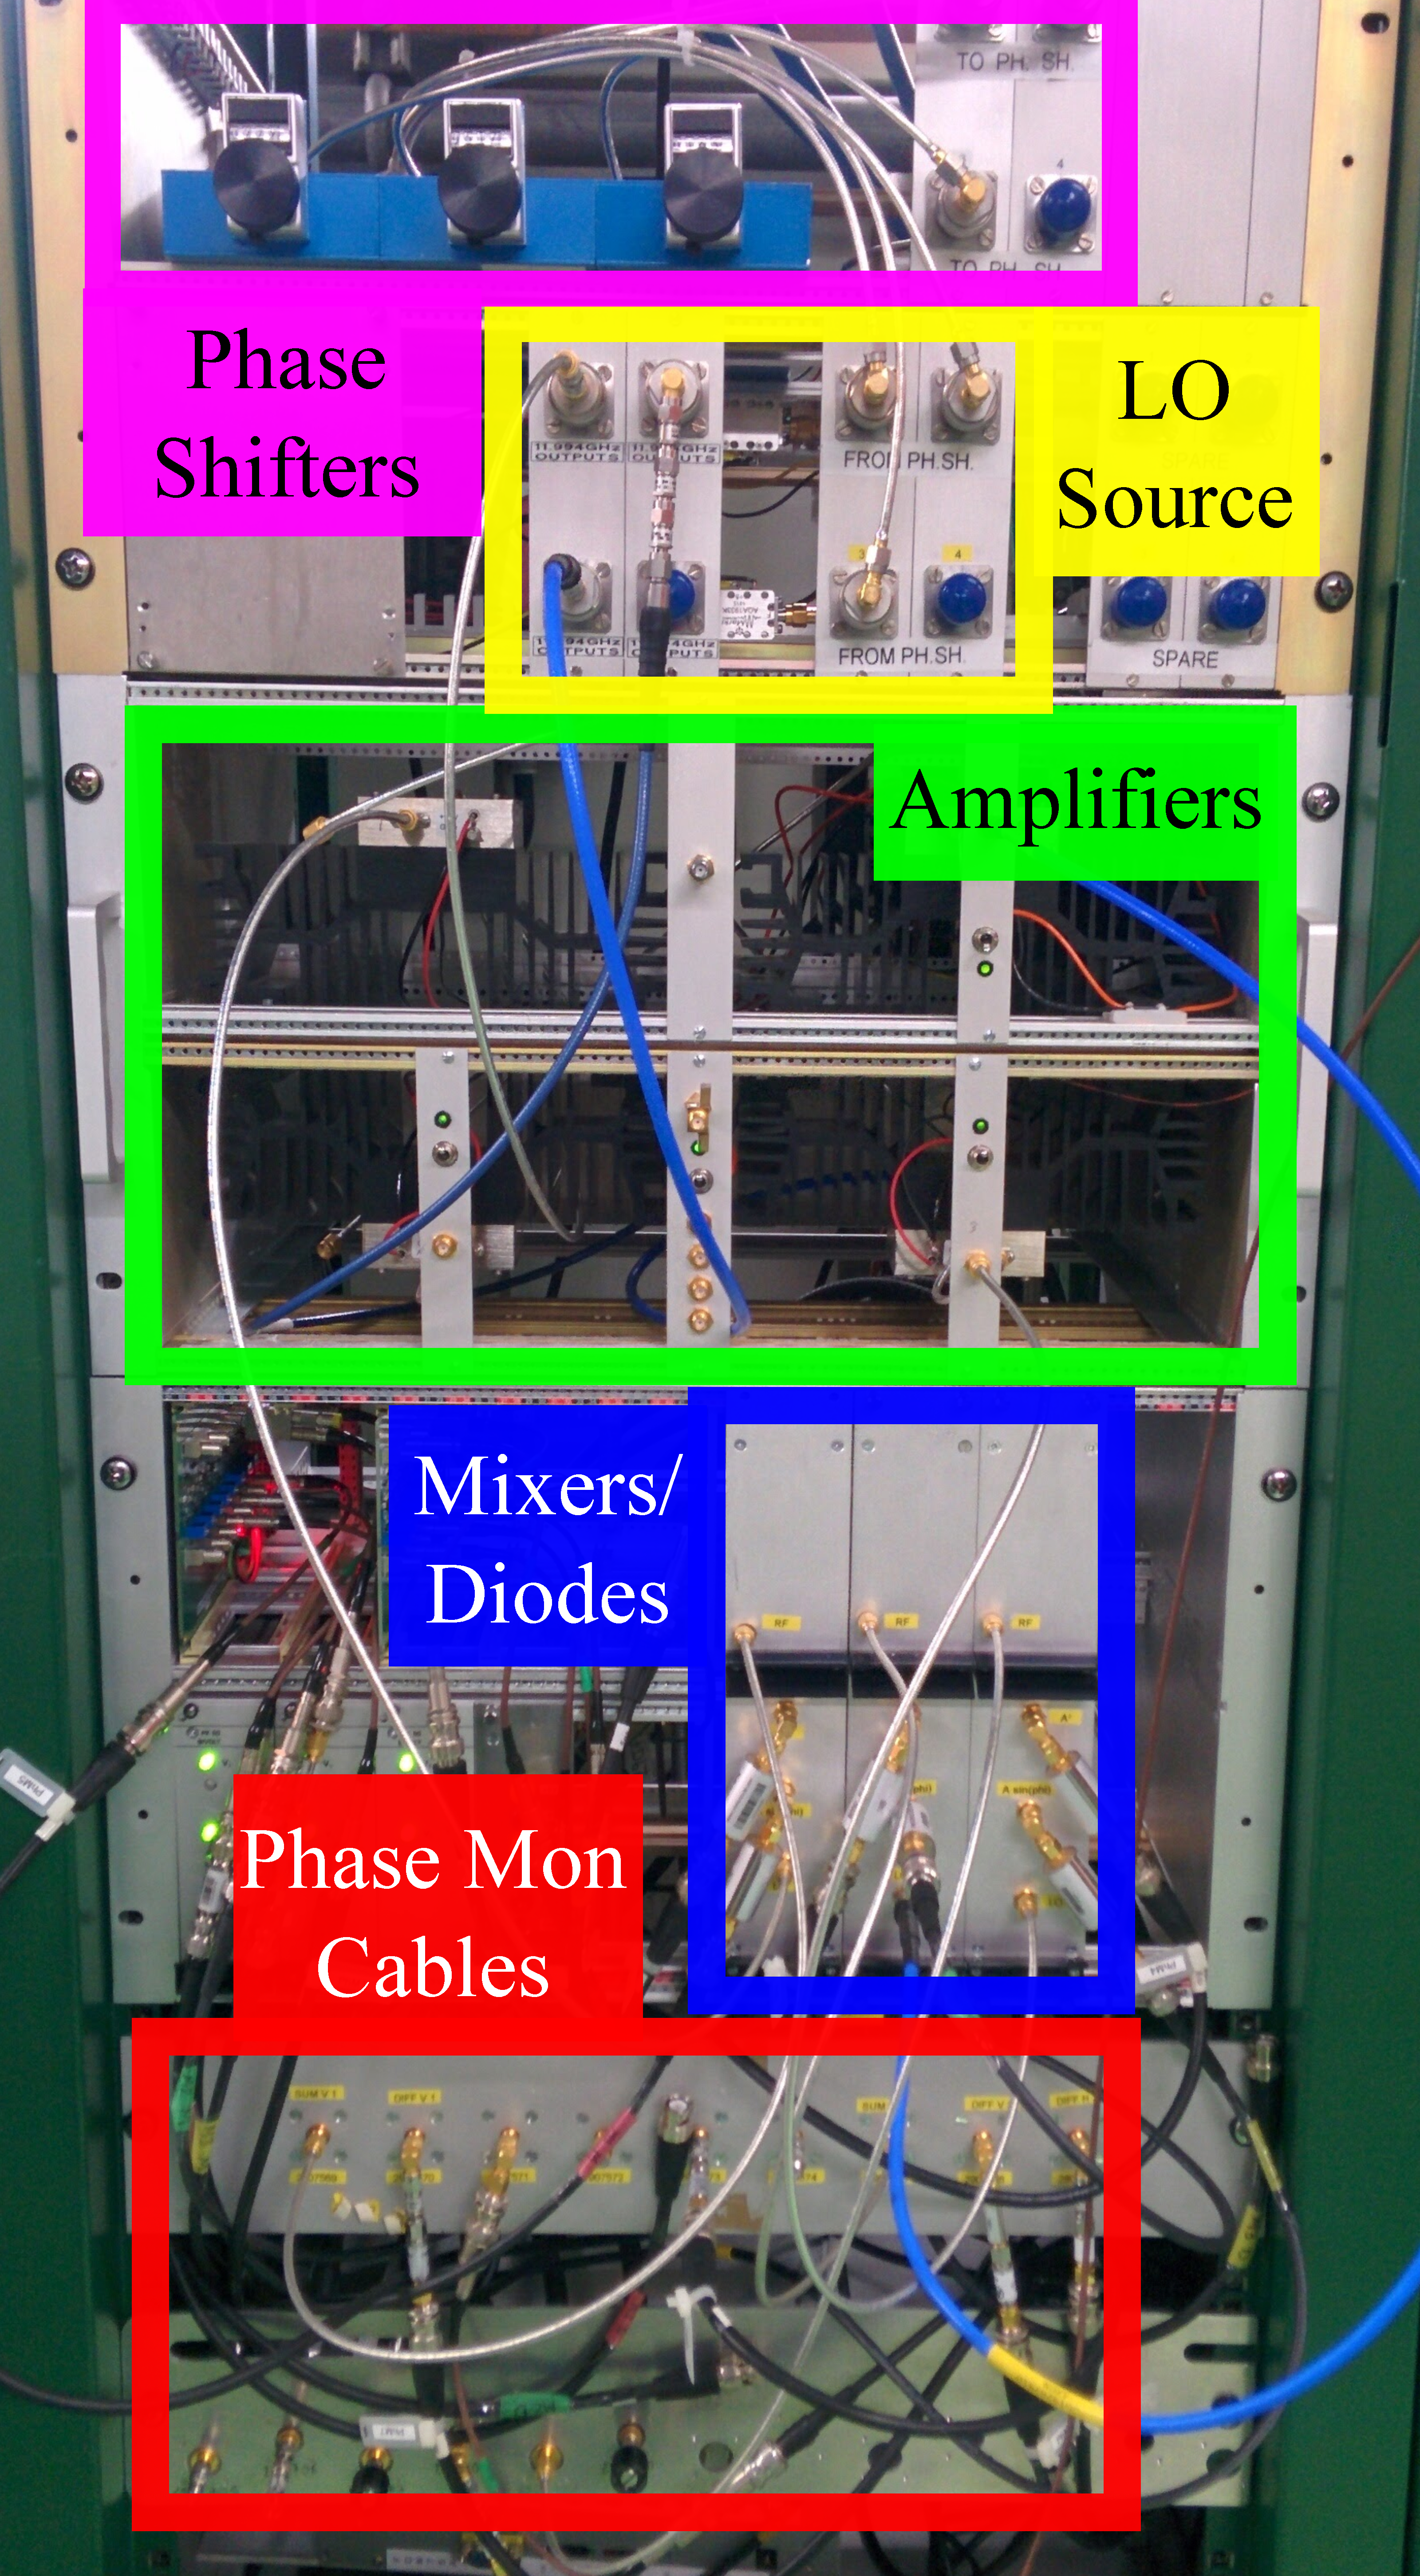
\includegraphics[width=\textwidth]{figs/hw/phMonRack}% Here is 
	%how to 
	%import EPS art
	\caption{\label{f:phMonRack}
	}
\end{figure*}

\begin{figure}
	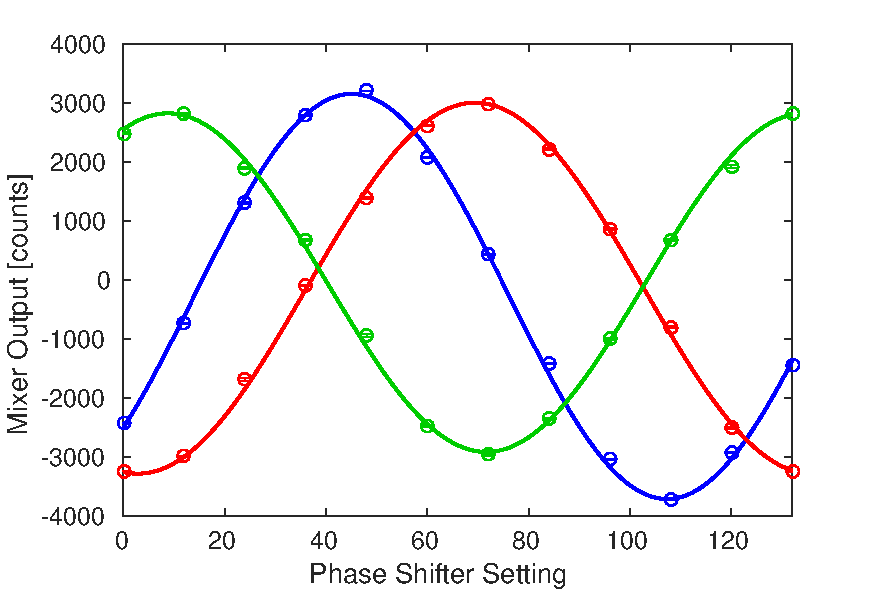
\includegraphics[width=\columnwidth]{figs/hw/phMonCal}% Here is 
	%how to 
	%import EPS art
	\caption{\label{f:phMonCal}
	}
\end{figure}

\begin{figure}
	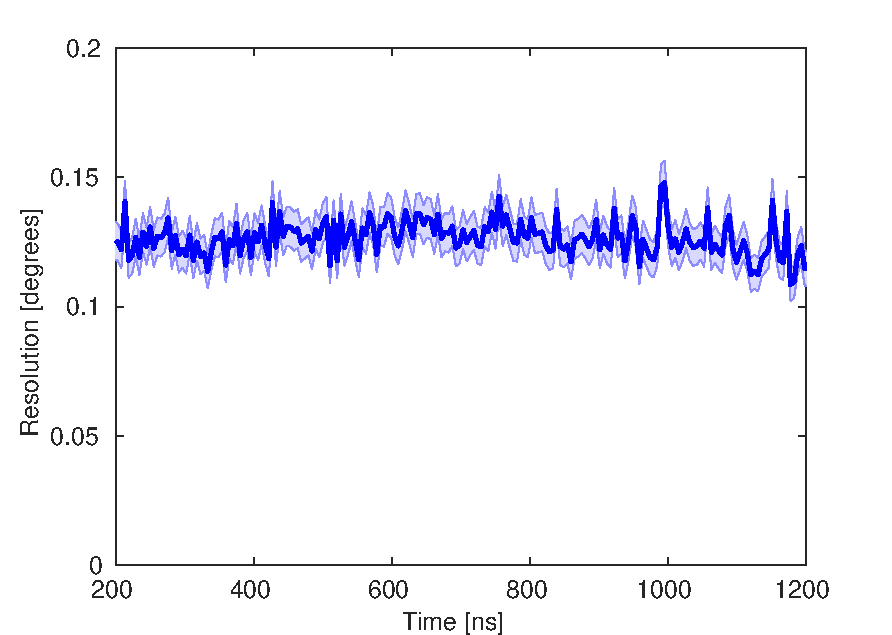
\includegraphics[width=\columnwidth]{figs/hw/phMonRes}% Here is 
	%how to 
	%import EPS art
	\caption{\label{f:phMonRes}
	}
\end{figure}

\begin{figure}
	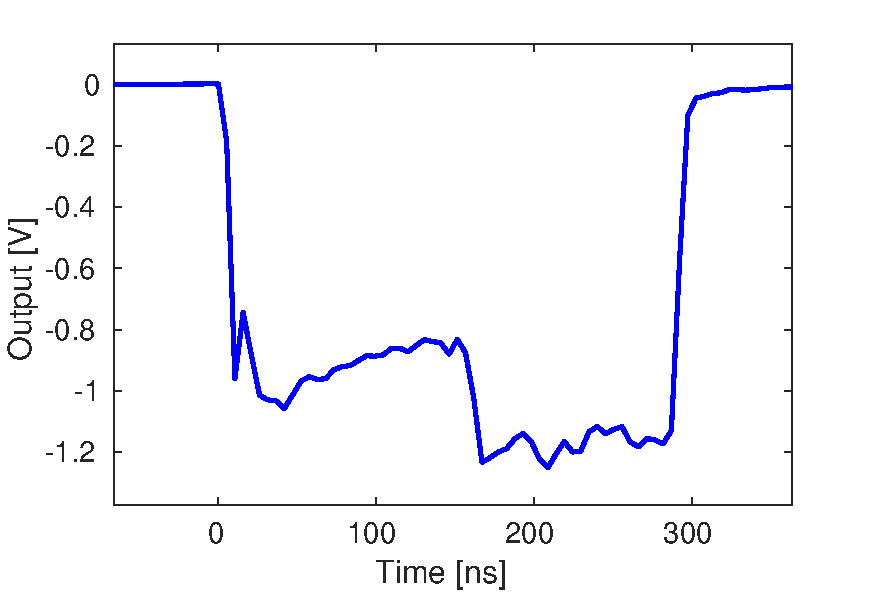
\includegraphics[width=\columnwidth]{figs/hw/phMonBw}% Here is 
	%how to 
	%import EPS art
	\caption{\label{f:phMonBw}
	}
\end{figure}

\begin{figure}
	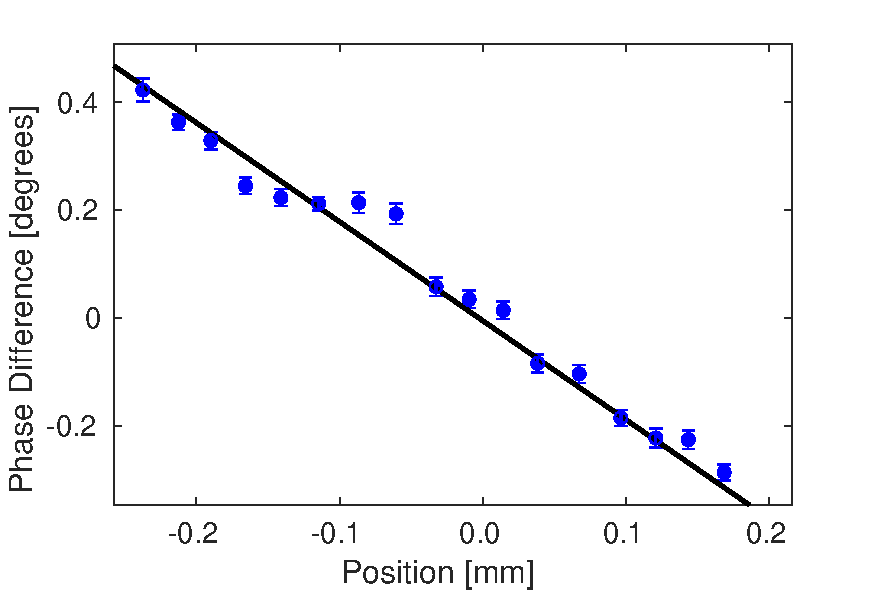
\includegraphics[width=\columnwidth]{figs/hw/phMonHScan}% Here is 
	%how to 
	%import EPS art
	\caption{\label{f:phMonHScan}
	}
\end{figure}

\subsection{\label{ss:kick}Kickers}

\begin{figure}
	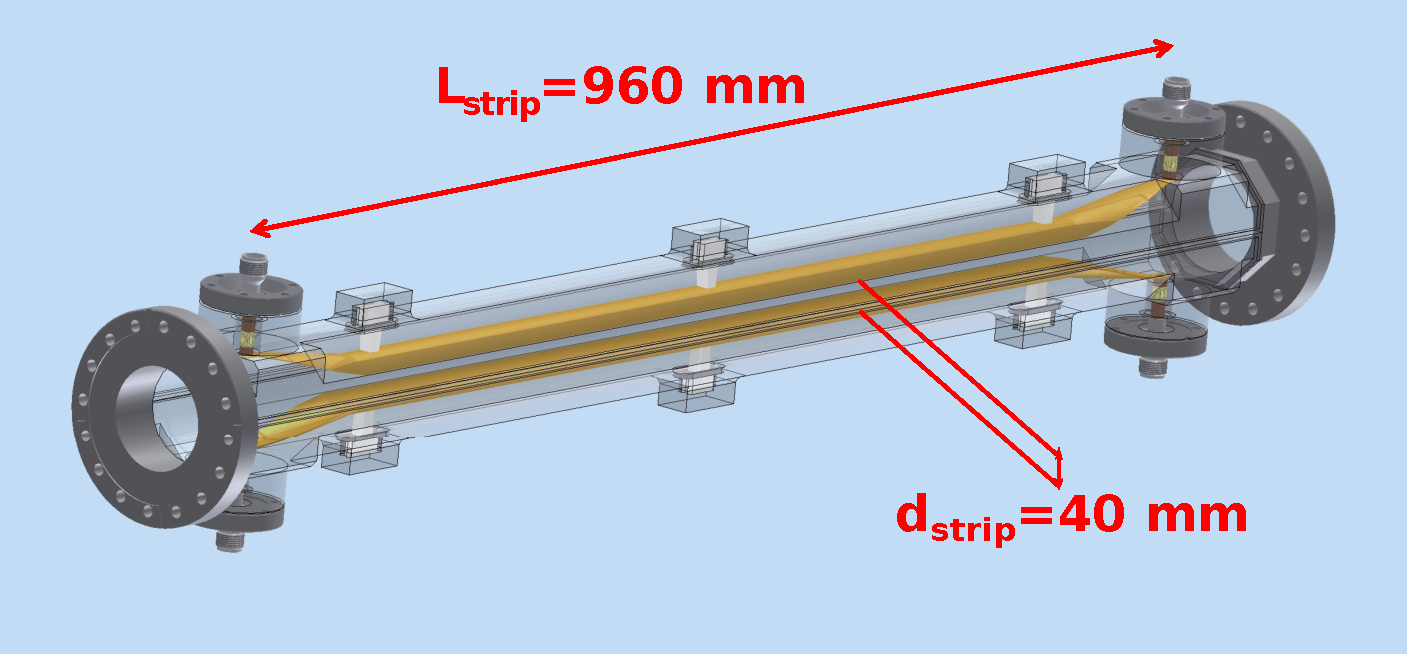
\includegraphics[width=\columnwidth]{figs/hw/kickerSchematic}% Here is 
	%how to 
	%import EPS art
	\caption{\label{f:kickerSchematic}
	}
\end{figure}

\subsection{\label{ss:amp}Amplifiers}

\begin{figure*}
	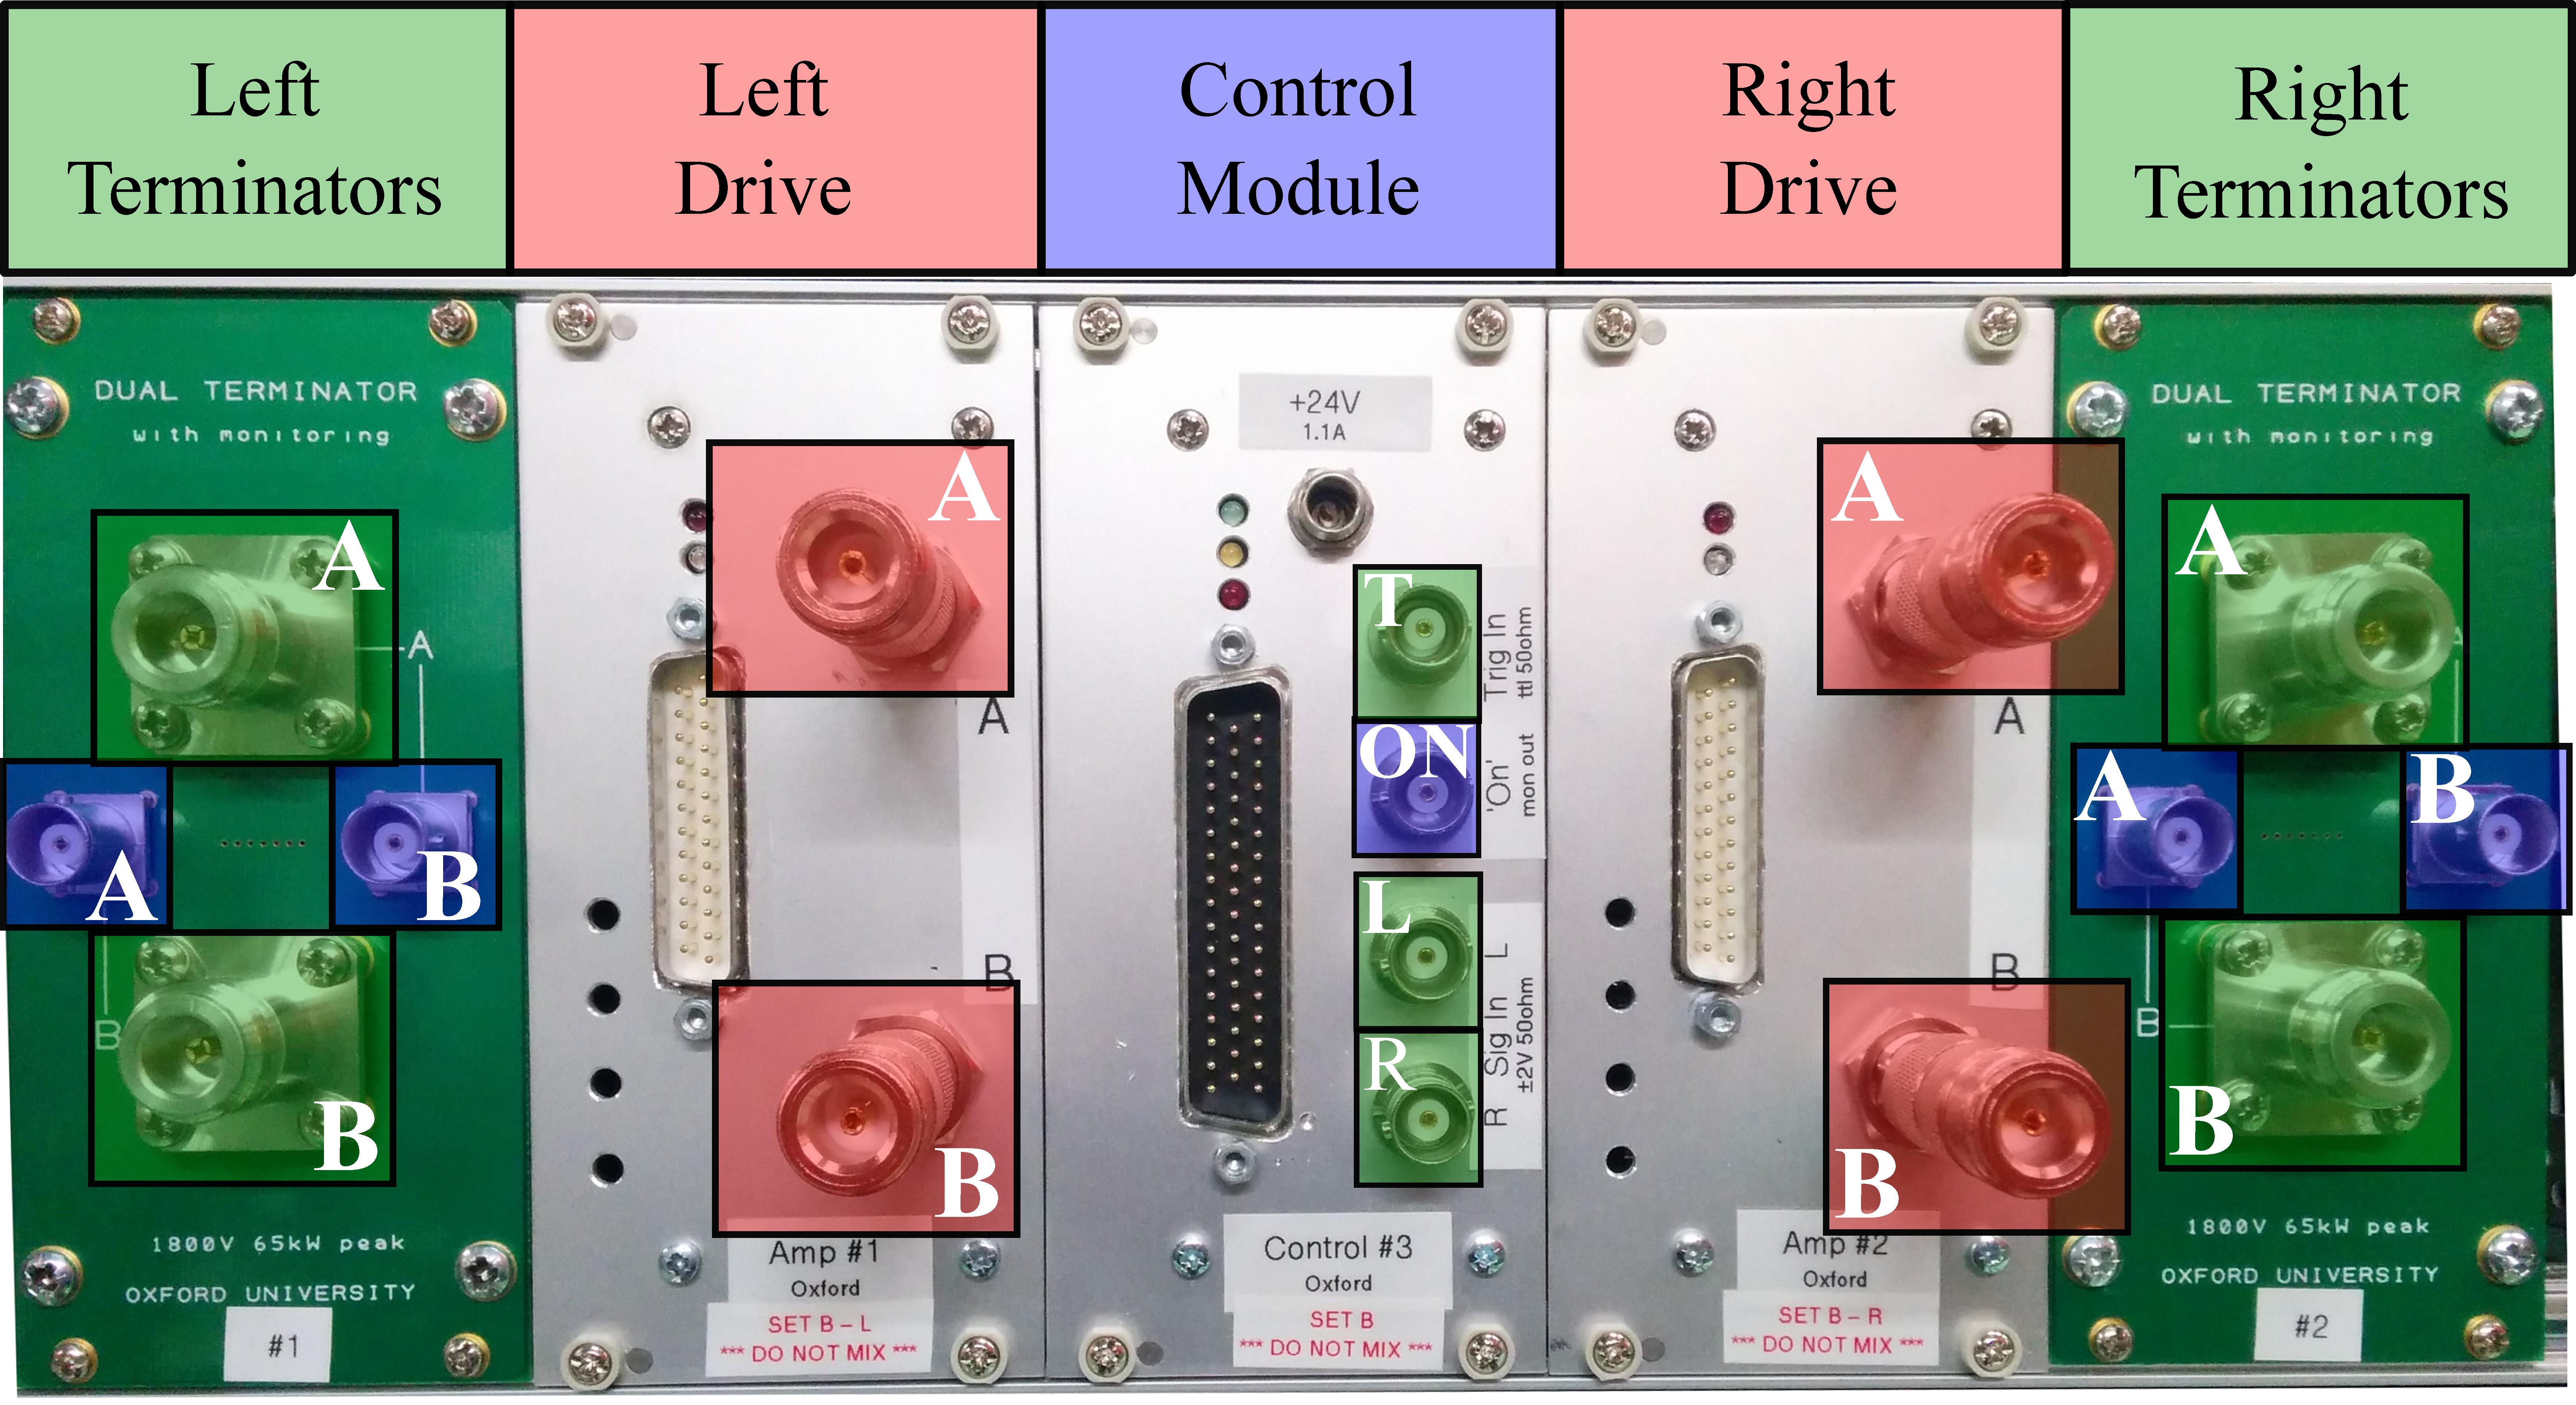
\includegraphics[width=\textwidth]{figs/hw/AmpPanel}% Here is 
	%how to 
	%import EPS art
	\caption{\label{f:AmpPanel}
	}
\end{figure*}

\begin{figure}
	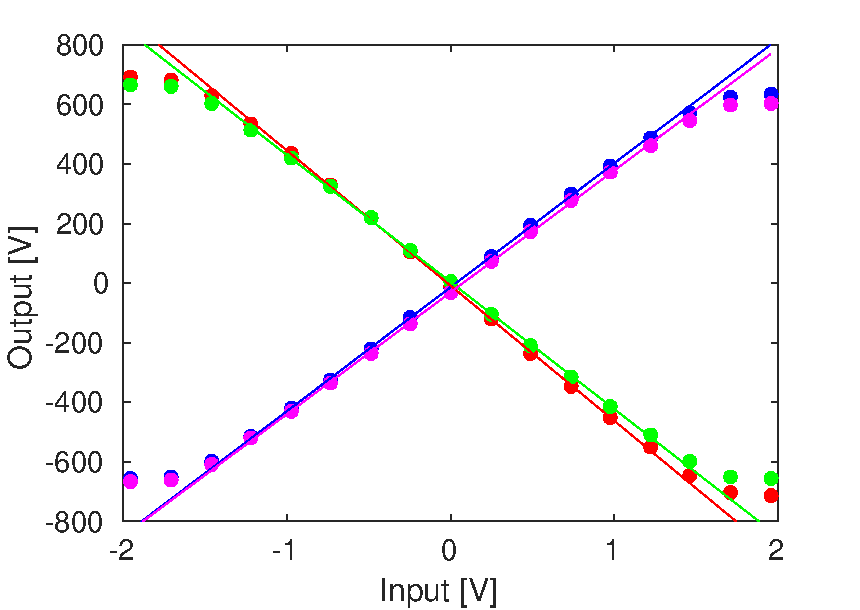
\includegraphics[width=\columnwidth]{figs/hw/AmpOutvsDAC}% Here is 
	%how to 
	%import EPS art
	\caption{\label{f:AmpOutvsDAC}
	}
\end{figure}

\begin{figure}
	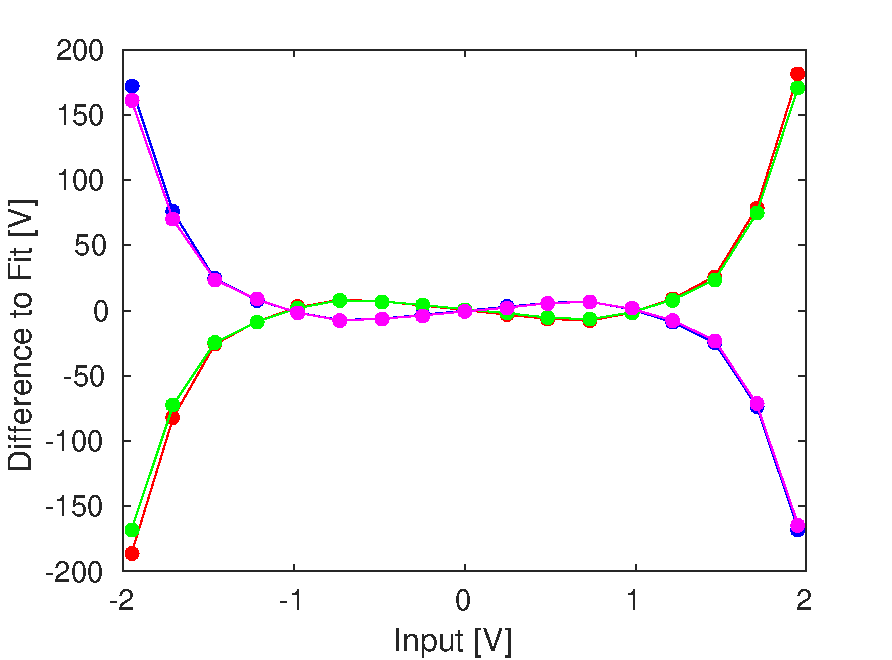
\includegraphics[width=\columnwidth]{figs/hw/AmpOutvsDAC_residual}% Here is 
	%how to 
	%import EPS art
	\caption{\label{f:AmpOutvsDAC_residual}
	}
\end{figure}


\begin{figure}
	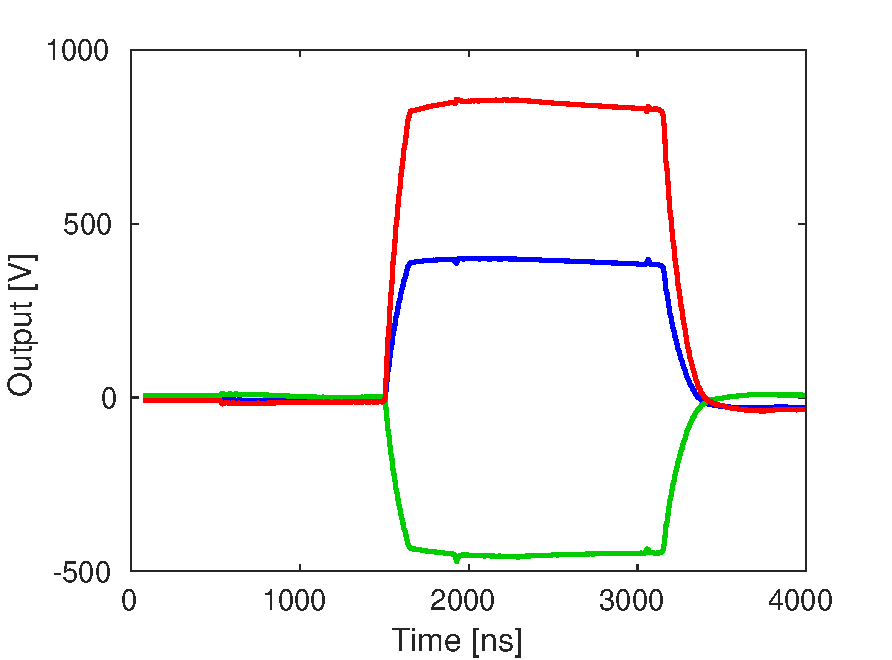
\includegraphics[width=\columnwidth]{figs/hw/AmpL_Traces}% Here is 
	%how to 
	%import EPS art
	\caption{\label{f:AmpL_Traces}
	}
\end{figure}

\subsection{\label{ss:font}Feedforward Controller}

\begin{figure}
	\includegraphics[width=\columnwidth]{figs/hw/FONT5aPanel}% Here is 
	%how to 
	%import EPS art
	\caption{\label{f:FONT5aPanel}
	}
\end{figure}

\begin{figure*}
	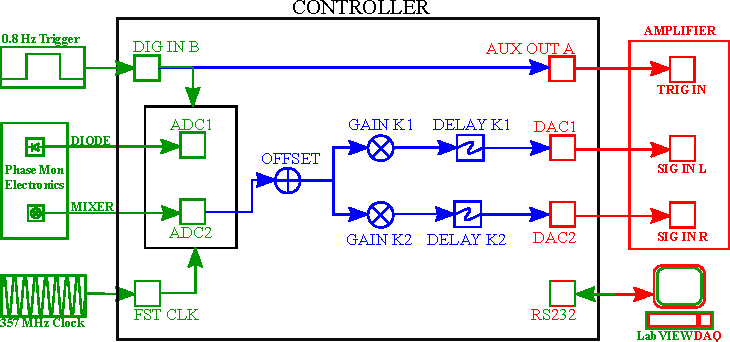
\includegraphics[width=\textwidth]{figs/hw/fontDiagram}% Here is 
	%how to 
	%import EPS art
	\caption{\label{f:fontDiagram}
	}
\end{figure*}

\section{\label{s:optics}Optics}

\begin{figure}
	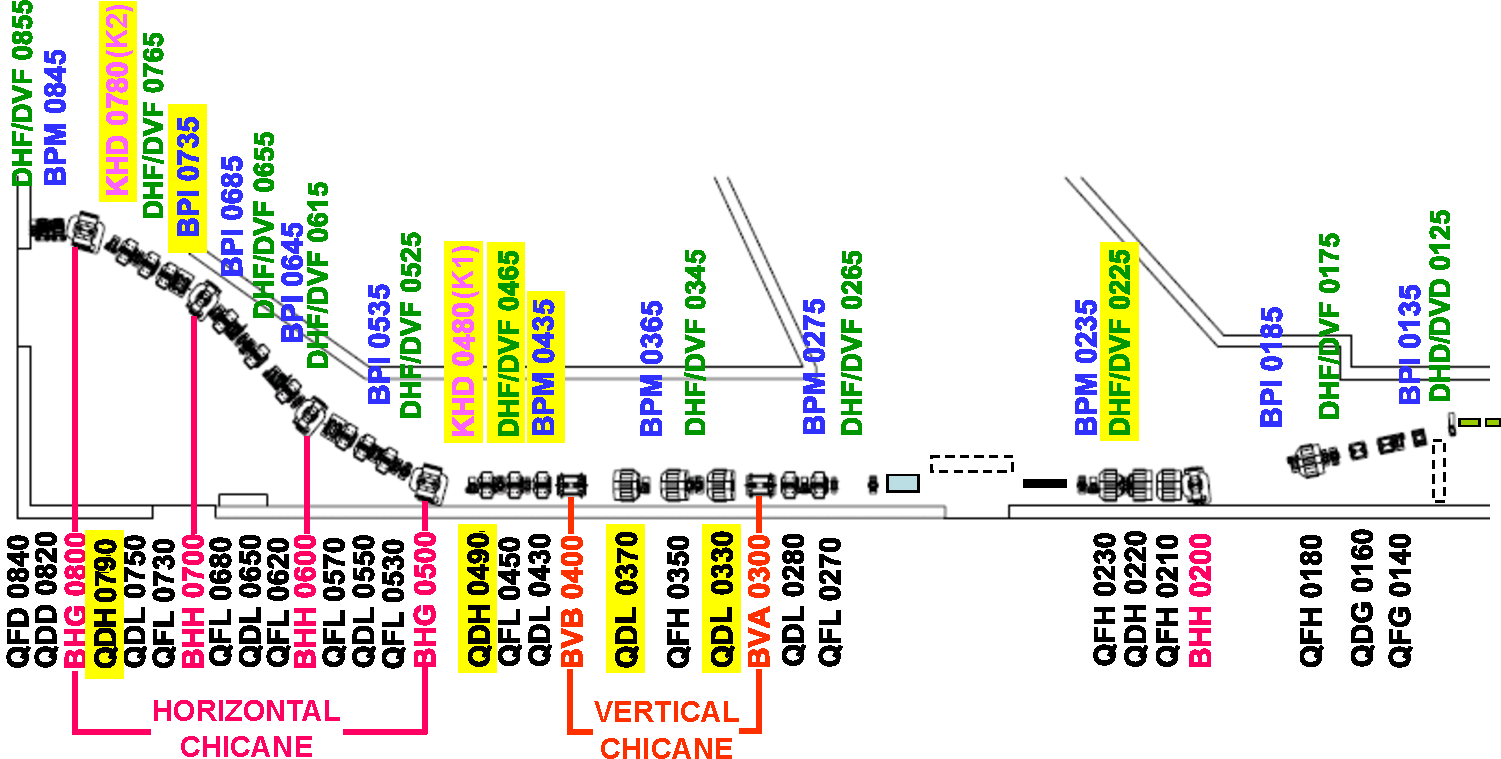
\includegraphics[width=\columnwidth]{figs/optics/TL2Lattice}% Here is 
	%how to 
	%import EPS art
	\caption{\label{f:TL2Lattice}
	}
\end{figure}

\begin{figure}
	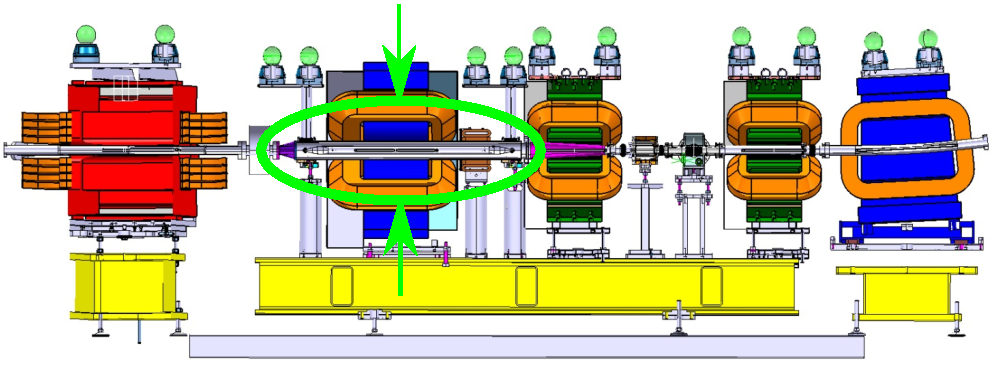
\includegraphics[width=\columnwidth]{figs/optics/kickerInsideQuad}% Here is 
	%how to 
	%import EPS art
	\caption{\label{f:kickerInsideQuad}
	}
\end{figure}

\begin{figure*}
	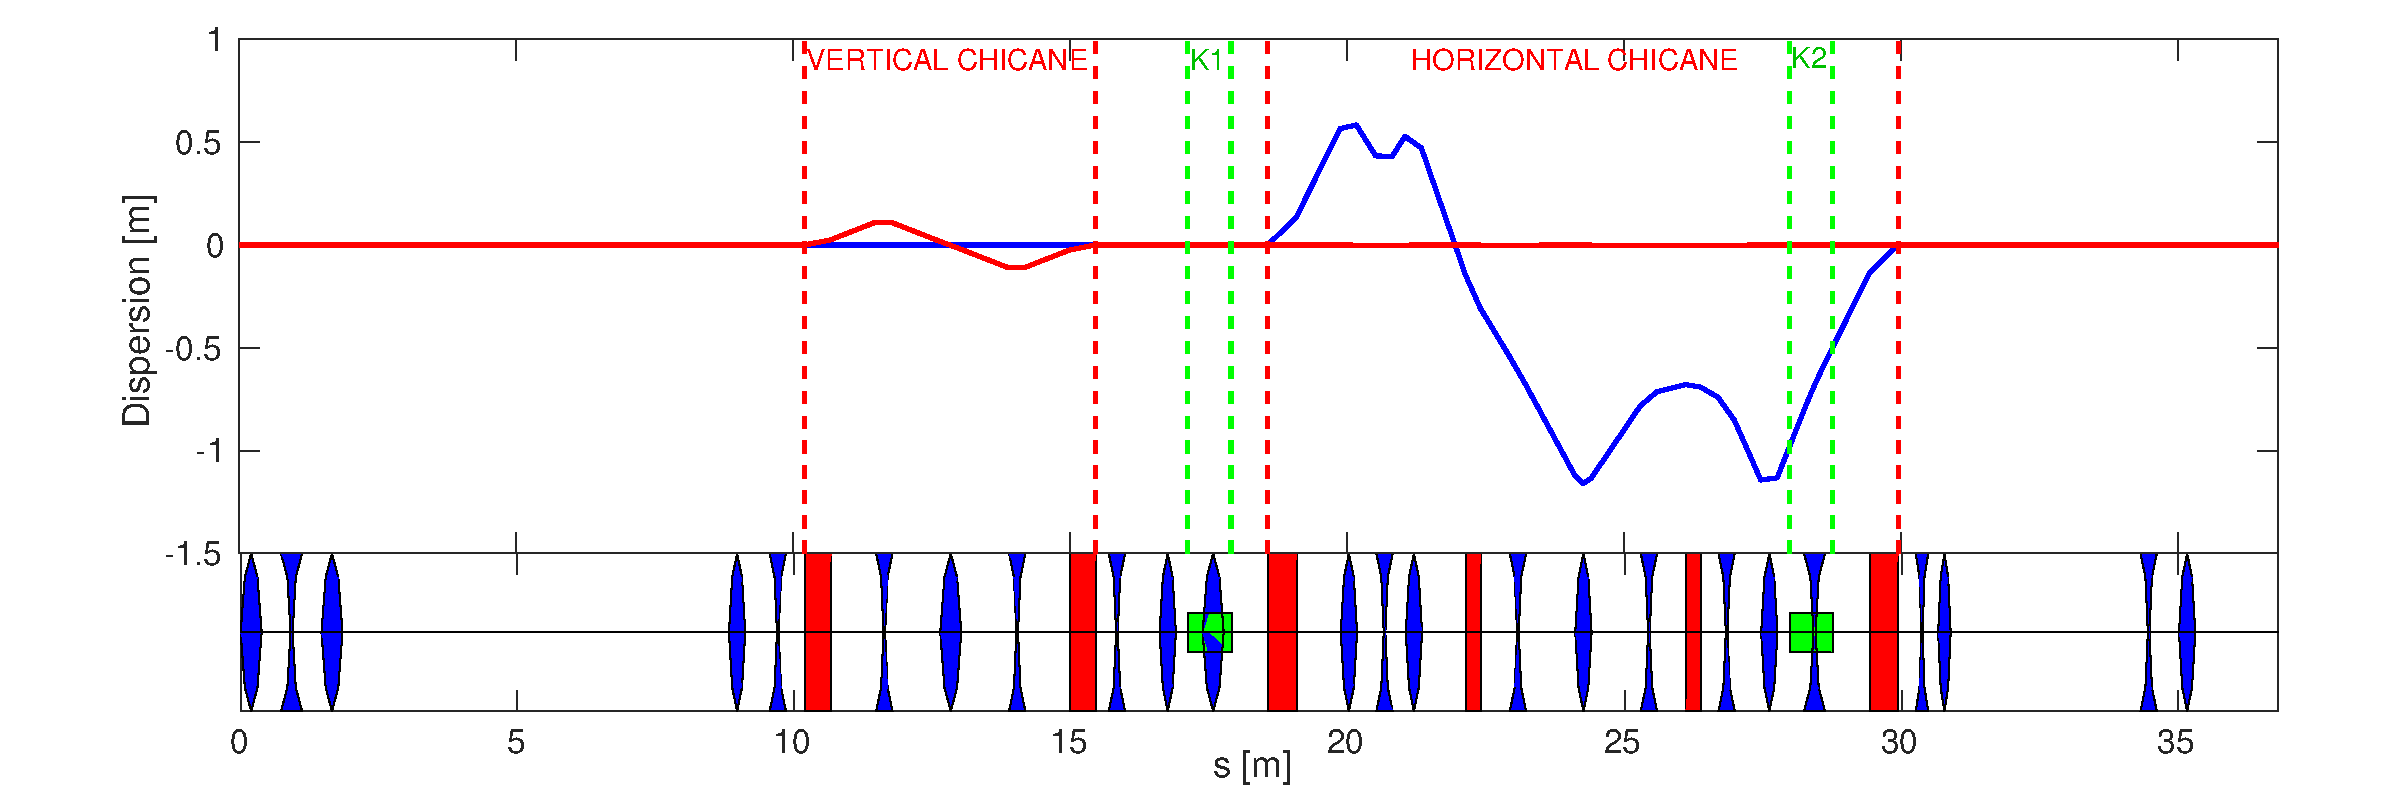
\includegraphics[width=\textwidth]{figs/optics/pffOpticsDisp}% Here is 
	%how to 
	%import EPS art
	\caption{\label{f:pffOpticsDisp}
	}
\end{figure*}

\begin{figure}
	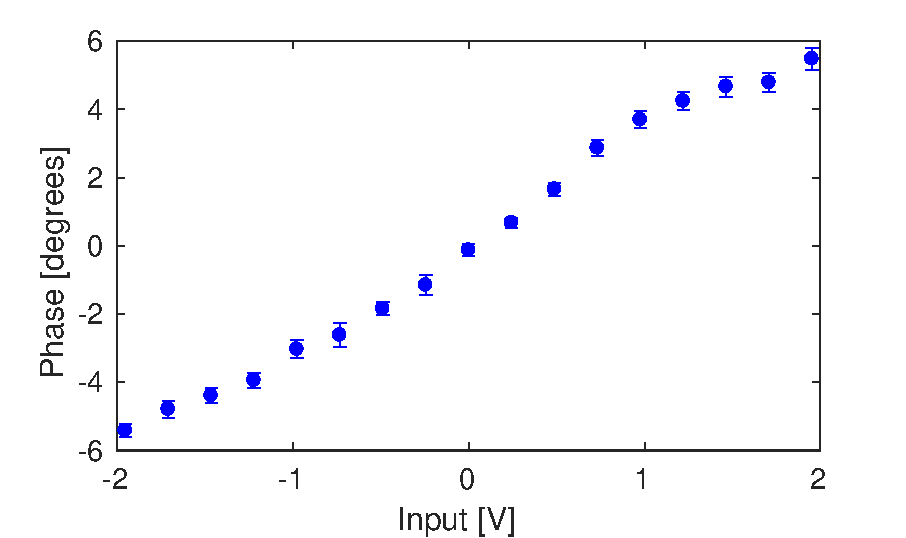
\includegraphics[width=\columnwidth]{figs/optics/corrRange}% Here is 
	%how to 
	%import EPS art
	\caption{\label{f:corrRange}
	}
\end{figure}

\begin{figure}
	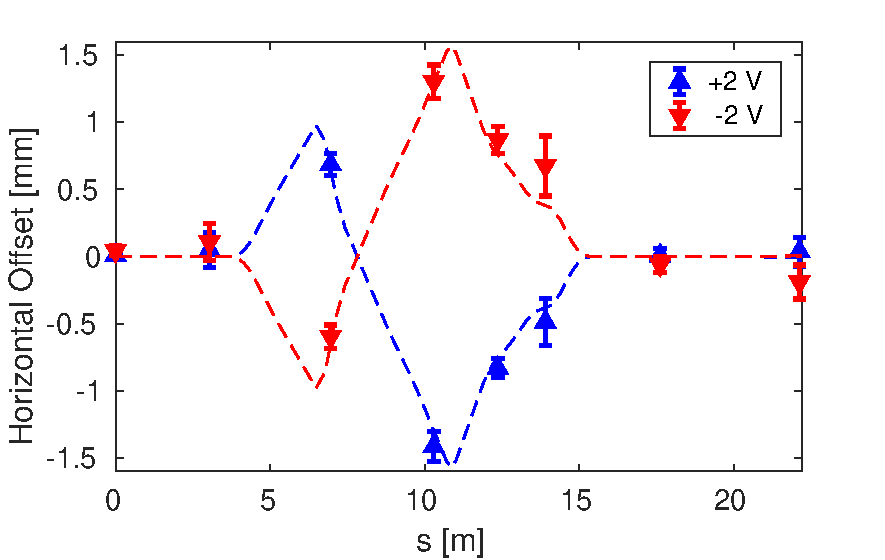
\includegraphics[width=\columnwidth]{figs/optics/orbClos}% Here is 
	%how to 
	%import EPS art
	\caption{\label{f:orbClos}
	}
\end{figure}

\section{\label{s:prop}Propagation}

\begin{figure}
	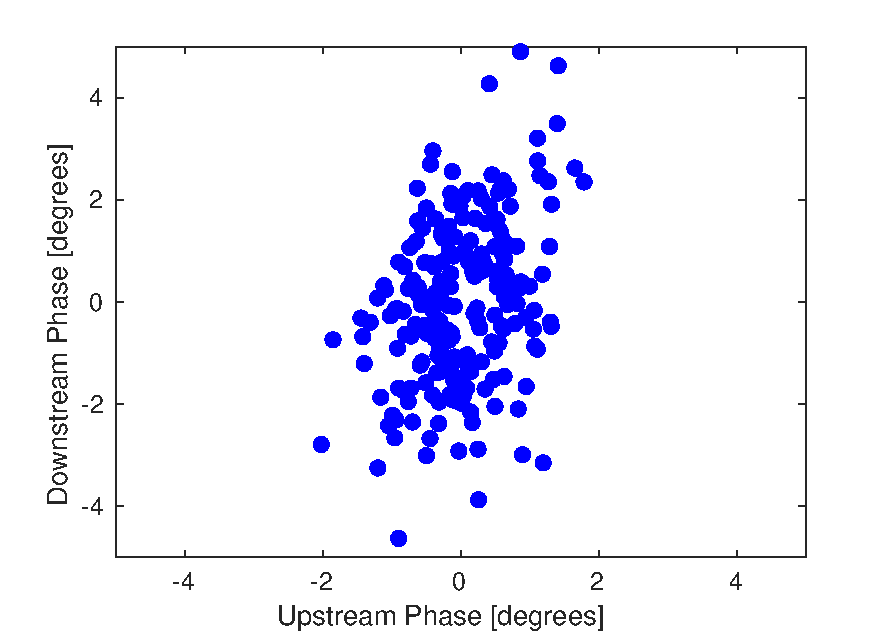
\includegraphics[width=\columnwidth]{figs/prop/origUpVsDown}% Here is 
	%how to 
	%import EPS art
	\caption{\label{f:origUpVsDown}
	}
\end{figure}

\begin{figure}
	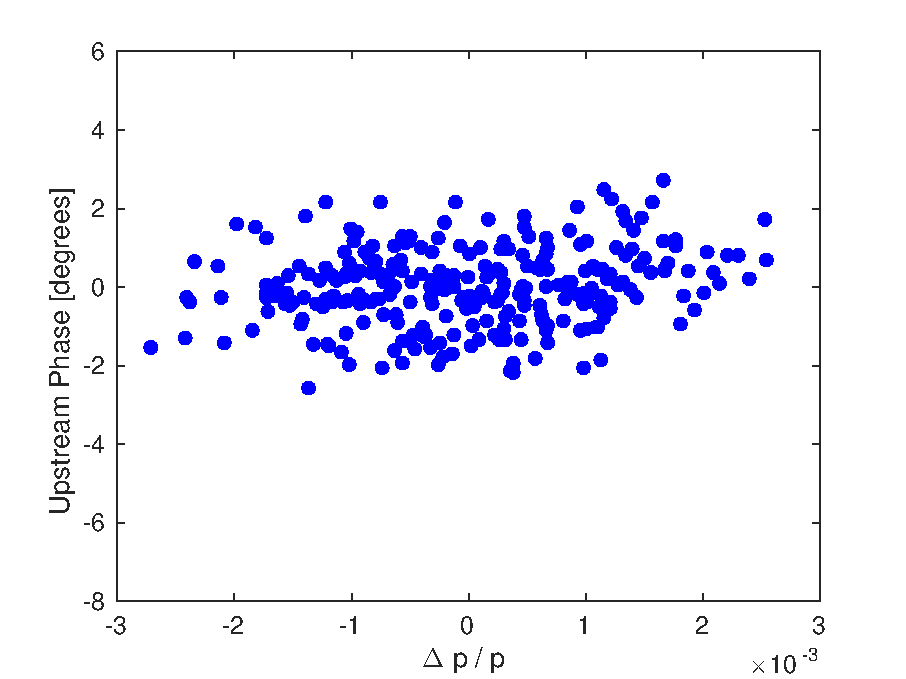
\includegraphics[width=\columnwidth]{figs/prop/corrUpstreamEn}% Here is 
	%how to 
	%import EPS art
	\caption{\label{f:corrUpstreamEn}
	}
\end{figure}

\begin{figure}
	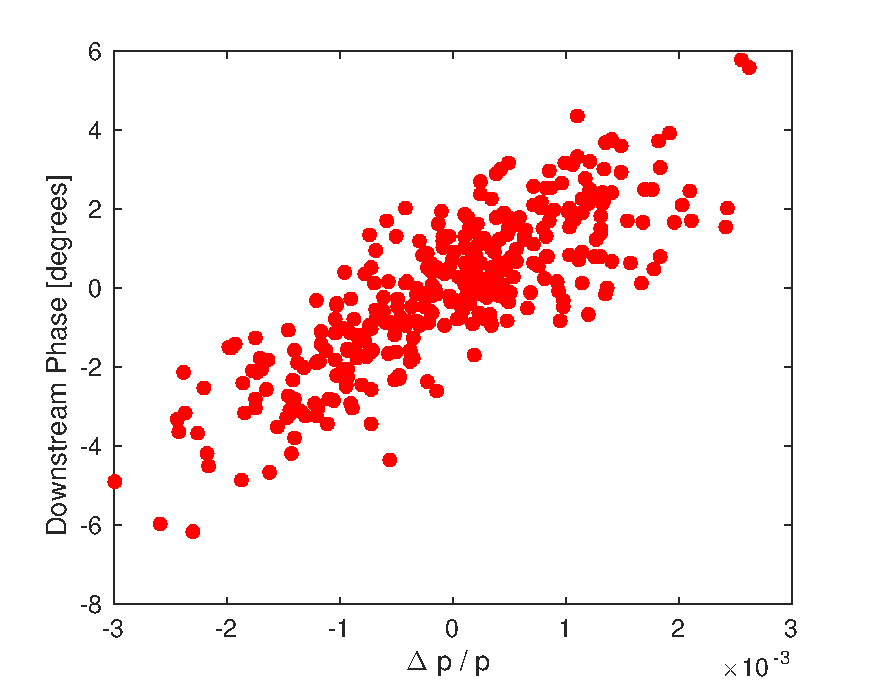
\includegraphics[width=\columnwidth]{figs/prop/corrDownstreamEn}% Here is 
	%how to 
	%import EPS art
	\caption{\label{f:corrDownstreamEn}
	}
\end{figure}

\section{\label{s:timing}System Latency and Timing}

The arrival time of the correction signal (drive voltage) and the beam at the 
two kickers must be precisely synchronised. The beam time of flight between the 
upstream phase monitors and the first kicker is 380~ns. In comparison, the 
total PFF system latency was estimated to be around 335~ns, with the largest 
contribution being the 175~ns signal transit time in the cables between the 
amplifiers and kickers. [TODO: Latency breakdown table?] The DAC output of the 
FONT5a board can be delayed in steps of 2.8~ns (the ADC clock frequency) to 
align the correction with the beam.

The required output delay has been verified by observing the amplifier 
monitoring signals and beam based measurements. The beam based approach is 
shown here. 

Large feature added to the intra-pulse phase by manipulating the waveform of 
klystrons in the CTF3 linac. The added phase variation is clearly visible in 
the upstream and downstream phase monitors. The correction is applied in 
interleaved mode, alternating between pulses with the correction on and off. 
The applied kick is calculated by taking the difference between the on and off 
pulses. The necessary delay can then be calculated by comparing the time of the 
phase bump in the original phase and in the applied kick.

\begin{figure}
	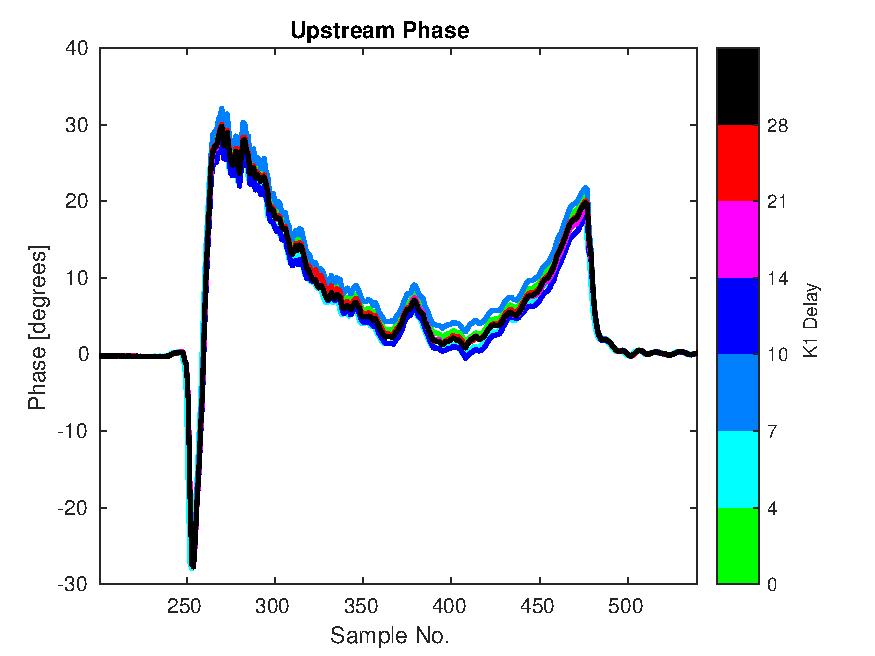
\includegraphics[width=\columnwidth]{figs/comis/bumpMon2}% Here is 
	%how to 
	%import EPS art
	\caption{\label{f:bumpMon2}
	}
\end{figure}

\begin{figure}
	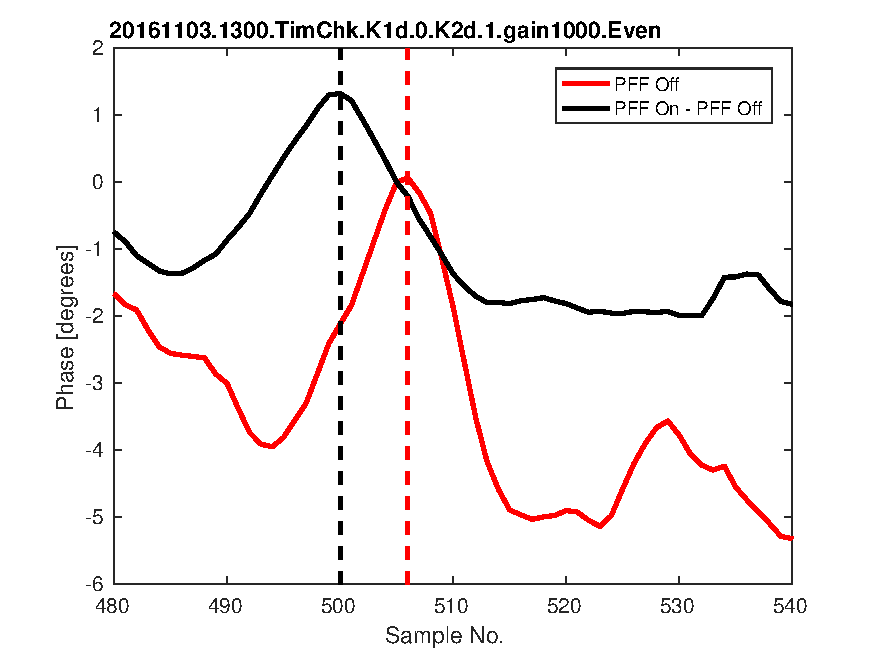
\includegraphics[width=\columnwidth]{figs/comis/bumpMon3}% Here is 
	%how to 
	%import EPS art
	\caption{\label{f:bumpMon3}
	}
\end{figure}

\begin{figure}
	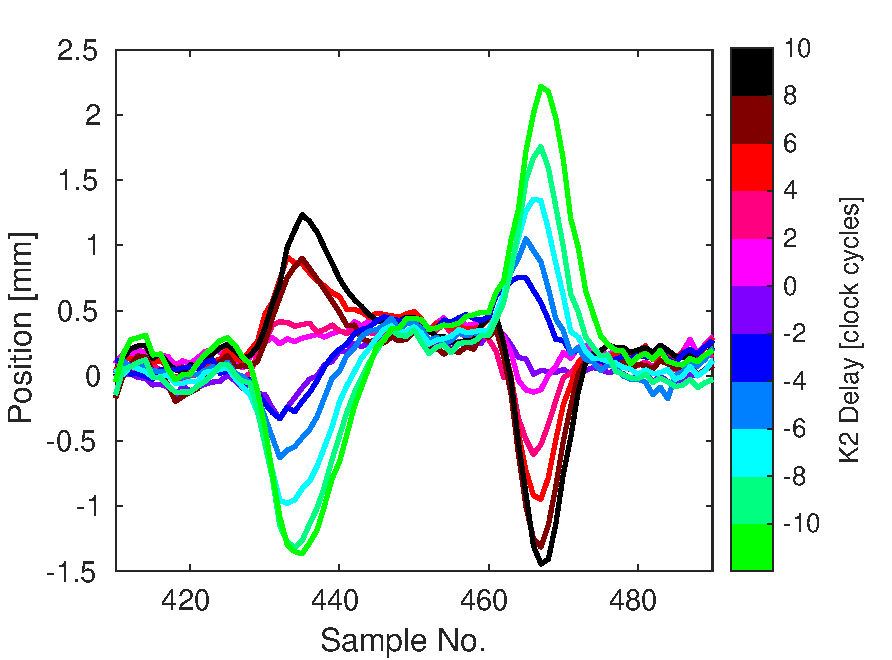
\includegraphics[width=\columnwidth]{figs/comis/relDelay_traces}% Here is 
	%how to 
	%import EPS art
	\caption{\label{f:relDelay_traces}
	}
\end{figure}

\begin{figure}
	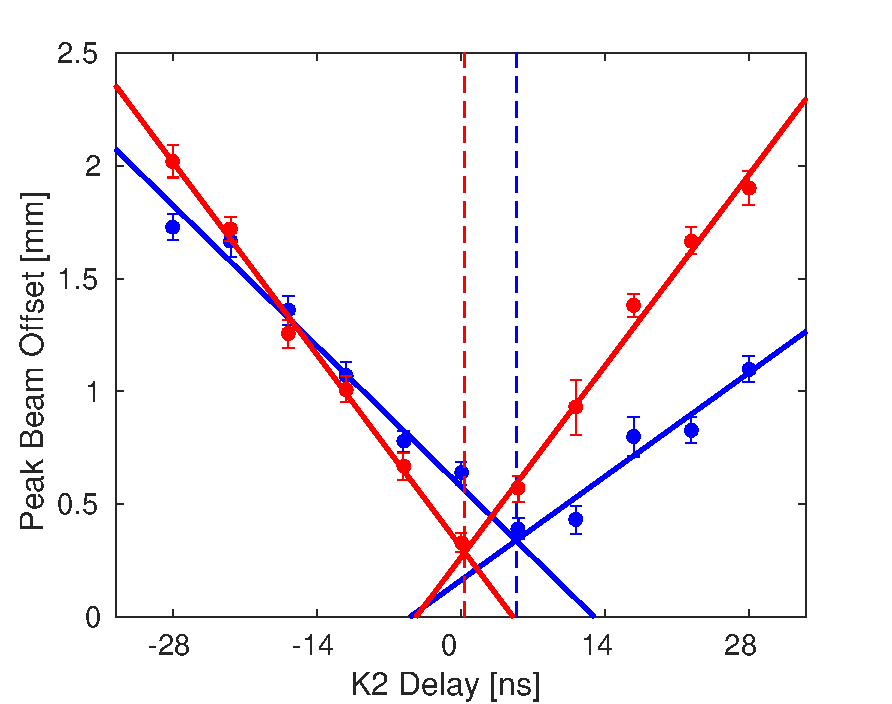
\includegraphics[width=\columnwidth]{figs/comis/relDelay_fit}% Here is 
	%how to 
	%import EPS art
	\caption{\label{f:relDelay_fit}
	}
\end{figure}

\section{\label{s:results}Results}


\section{\label{s:conc}Conclusions}

\begin{acknowledgments}
	We wish to acknowledge Alessandro Zolla and Giancarlo Sensolini (INFN 
	Frascati) for their work on the mechanical design of the phase monitors and 
	kickers, 
	Alexandra Andersson, Luca Timeo and Stephane Rey (CERN) for their work on 
	the phase monitor electronics, and everyone involved in the operation of 
	CTF3 for their help and support in realising the PFF system.
\end{acknowledgments}

\bibliography{pff_prab}

\end{document}
